\documentclass[11pt,letterpaper]{article}
\usepackage[utf8]{inputenc}
\usepackage[T1]{fontenc}
\usepackage[spanish]{babel}
\usepackage[left=2.54cm,top=2.54cm,right= 2.54cm, bottom=2.54cm]{geometry}
\usepackage{amsmath}
\usepackage{amsfonts}
\usepackage{amssymb}
\usepackage{enumerate}
\renewcommand{\baselinestretch}{2}
\usepackage{graphicx}
\graphicspath{{Figuras/}}
\usepackage{float}
\begin{document}
\begin{center}
TRASNFORMADA DE LAPLACE, INTEGRAL DE CONVOLUCION Y EJERCICIOS DE APLICACIÓN\vspace{3cm}


PRESENTADO POR:\\
SEBASTIÁN VELASCO LÓPEZ\vspace{1.5cm}

TUTOR:\\
JHONATAN COLLAZOS\vspace{2.5cm}

CURSO INTERSEMESTRAL DE ECUACIONES DE VERANO
\vspace{3cm}

FACULTAD DE INGENIERÍA CIVIL\\
UNIVERISDAD DEL CAUCA SEDE POPAYAN.\vspace{2.5cm}
 
Popayan Cauca.\\
29 de agosto de 2022\\

\end{center}
\newpage
\section{INTRODUCCIÓN}
La transformada de Laplace es una técnica, empleada tanto en ingeniería como en ciencias, para resolver ecuaciones diferenciales lineales con coeficientes constantes y condiciones iniciales. En el siguiente trabajo se dará una definición de la transformada de Laplace y su explicación matemática con uno de sus teoremas derivados que es la integral de convolución y un ejercicio de aplicación el
cual se va a verificar en Matlab para dar una demostración de su comportamiento y dar veracidad
a la teoría de su aplicación.\\
\section{RESUMEN}
Dentro del documento se encuentra una breve historia de cómo surgió la transformada de Laplace y su inventor, al igual que su definición y su explicación matemática, lo cual nos va a permitir captar o tener una idea de lo que es la transformad de Laplace en las ecuaciones diferenciales y explicar uno de sus tatos teoremas como lo es en este caso la integral o teorema de convolucion en donde se podrá observar 4 casos diferentes para obtener un resultado final y llegar a una convolucion y observar el comportamiento de una función o ejercicio el cual vamos a probar por medio de Matlab y sus aplicaciones y comprobar el funcionamiento y comportamiento de este
ejercicio.\\
Simón marques de Laplace fue matemático y astrónomo francés famoso en su tiempo conocido en
su tiempo como el newton e Francia, sus campos principales fueron la mecánica celeste o
movimiento planetario, teoría de probabilidades y el progreso personal.\\
 La transformada de Laplace es una técnica matemática que forma parte de ciertas transformadas integrales como la transformada de Fourier, la trasformada de Hilbert, y la transformada de Mellin, entre otras. Estas transformadas están definidas por medio de una integral impropia y
cambian una función en una variable de entrada en otra función en otra variable. 
\\La transformada de Laplace puede resolver ecuaciones diferenciales lineales y ecuaciones
integrales.\\Se pueden resolver algún tipo de ecuaciones diferenciales con coeficientes variables y en general se aplica a problemas con coeficientes constantes. Un requisito adicional es el conocimiento de las
condiciones iniciales a la misma ecuación diferencial.\\Su mayor ventaja sale a relucir cuando la función en la variable independiente que aparece en l aecuación diferencial es una función seccionada.\\
Se utiliza también en sistemas de control para obtener la función de transferencia y predecir o analizar el funcionamiento del sistema.\\
\section{LA TRANSFORMADA DE LAPLACE}
La definición de la transformada nos dice que sea $f$ una función definida para T mayor o igual que
$0$, la transformada de Laplace de $f(t)$ se define como la transformada de Laplace va a ser de $f(t)= \overset{+ \infty }{\underset{0}{\int }} e^{s-t} f(t)dt $ cuando la integral converja, debemos tener en cuenta que la letra S representa
una nueva variable que para el proceso de integración se considera constante, también que la transformada de Laplace convierte una función en $t$ en una función en la variable $s$

Debemos tener en cuenta que la existencia de la transformada tiene unas condiciones que nos
dice que las condiciones suficientes para la existencia de la transformada de Laplace nos dice que $S > \Delta$ de una función cualquiera, la primera cosa que debemos tener en
cuenta es que esta debe estar definida y ser continua a pedazos en el intervalo desde $(0; +\infty)$ y la segunda es que debe ser de orden exponencial.\\
\section{LA TRASNFORMADA INVERSA}
La definición de la transformada inversa nos dice que la transformada inversa de una función en $S$
digámoslo así, $F$ mayúscula de $S$ es una función de $T$ cuya transformada es precisamente $F$ mayúscula de $S$, es decir que la inversa, por eso esta aquí $L^{-1}$, la inversa de Laplace
va a ser igual en este caso en este caso a $F$ mayúscula de $S$ igual a $f$ minúscula de T, si es que acaso la transformada de Laplace es igual a $f(t)$ minúscula, esta va a ser igual a $F (S)$,esta definición obliga a que se cumpla que la transformada de Laplace va a ser igual a al inversa de la transformada de Laplace de $F$ mayúscula de $S$ igual a $F$ mayúscula de $S$ o tenemos también que la transformada de Laplace va a ser igual a la transformada de Laplace de $F$ minúscula de $T$ igual a
$F$ minúscula de $T$\\
\textbf{LA TRANSFORMADA INVERSA DE UNA FUNCION EN S, DIGAMOS $F(S)$ ES UNA FUNCION DE T CUYA
TRANSFORMADA ES PRECISAMENTE $f(s)$, ES DECIR}
\begin{align}
L^{-1} [f(s)]= f(t)
\end{align}
Si es que acaso
\begin{align}
L [f(f)] = f(s)
\end{align}
Esta definicion pbliga a que se cumpla
\begin{align}
L \lbrace L^{-1} [f(s)] \rbrace = f(s)
\end{align}
Y
\begin{align}
L \lbrace L^{-1} [f(s)] \rbrace = f(s)
\end{align}
\newpage
\section{TEOREMA DE CONVOLUCIÓN}
En matemática, el teorema de convolución establece que, bajo determinadas
circunstancias, la transformada de Fourier de una convolución es el producto punto a punto (o producto Hadamard) de las transformadas.\\
$F(\tau)=$
\begin{figure} [H]
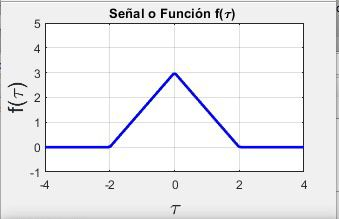
\includegraphics[scale=0.5]{figura 1}
\end{figure}
\begin{align}
(\frac{3}{2} t + 3) ; -2 < t < 0\\
(-\frac{3}{2} t + 3) ; 0 \leq t < 2 
\end{align}
\begin{center}
$0$ ; otro caso
\end{center}
\begin{figure} [H]
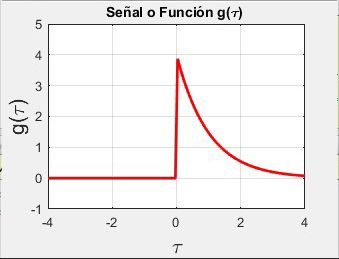
\includegraphics[scale=0.5]{figura 2}
\end{figure}
\begin{align}
g(\tau) = 4 e^{-t}u(t)
\end{align}
\newpage
Siguiendo con el ejemplo, por un lado tenemos una función $f (\tau)$ y escrita por un modelo de una
función a trozos $(5)$ y la gráfica que la acompaña, pero tenemos por otro lado a la
función denominada $g (t)$\\
$f(\tau)$
\begin{figure} [H]
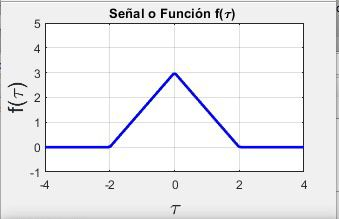
\includegraphics[scale=0.5]{figura 1}
\end{figure}
\begin{align}
\left( \frac{3}{2}\tau + 3 \right) ; -2 < \tau < 0\\
\left( -\frac{3}{2}\tau + 3 \right) ; 0 \leqslant \tau < 2
\end{align}
\begin{center}
0 ; otro caso
\end{center}
\begin{figure} [H]
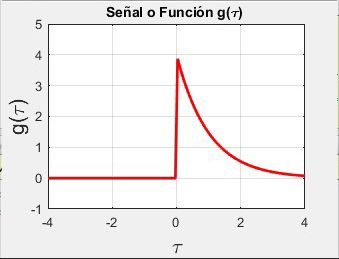
\includegraphics[scale=0.5]{figura 2}
\end{figure}
\begin{align}
g(\tau) = 4 e^{-\tau} \mu (\tau)
\end{align}
Luego escogemos una de las dos señales\\
\begin{figure} [H]
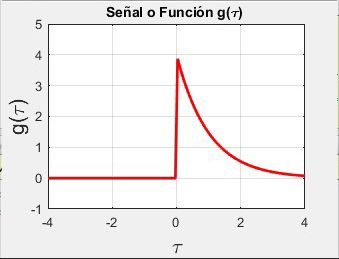
\includegraphics[scale=0.5]{figura 2}
\end{figure}
\begin{align}
g(-\tau) = 4 e^{-(-\tau)} \mu (-\tau)
\end{align}
Luego hacemos que la señal que elegimos, se traslade
\begin{figure} [H]
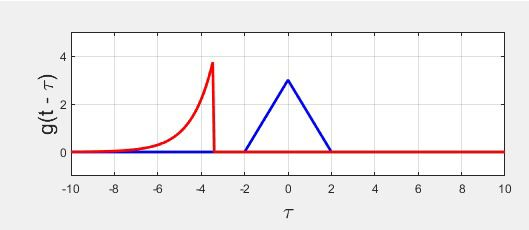
\includegraphics[scale=00.5]{figura 3}
\end{figure}
\begin{align}
g(t-\tau) = 4e^{-(t-\tau)} \mu (t - \tau)
\end{align}
Finalmente llegamos al paso donde aplicamos la definición de convolucion, que es la integral\\
\textbf{CASO (1)}\\
\begin{align}
y(t) = \overset{\infty}{\underset{-\infty}{\int }} f(\tau) g (t - \tau)dt
\end{align}
\begin{figure} [H]
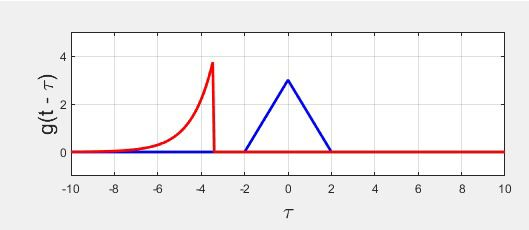
\includegraphics[scale=0.5]{figura 3}
\end{figure}
$y(t)=0\\
t<-2$\\
\textbf{CASO (2)}
\begin{figure} [H]
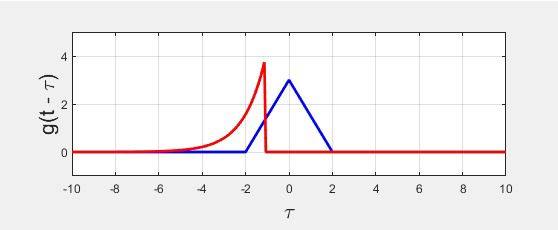
\includegraphics[scale=0.5]{figura 4}
\end{figure}
$t>-2 \wedge t<0\\
-2<t<0$
\begin{align}
y(t) = \overset{t}{\underset{-2}{\int }} \left[ \frac{3}{2} \tau + 3 \right] \left[ 4e^{-(t-\tau)} \right]d\tau\\
= 4e^{-t} \left[ \left( \frac{3}{2} \tau + 3 \right) e^\tau - \frac{3}{2} e^\tau \right] \mid^t _-1\\
= 4e^-t  \left( \frac{3}{2}t + 3 \right) e^t - \frac{3}{2} e^t - \left[ \left( \frac{3}{2} (-2) + 3  \right) e^{-2} - \frac{3}{2} e^{-2}  \right]
\end{align}
\textbf{CASO (3)}\\
\begin{figure} [H]
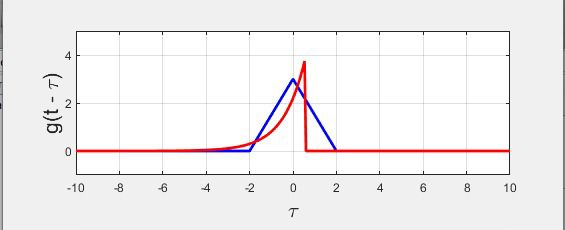
\includegraphics[scale=0.5]{figura 5}
\end{figure}
$t>o \wedge t < 2\\
0<t<2$
\begin{align}
y(t) = \overset{0}{\underset{-2}{\int }} \left[ \frac{3}{2} \tau + 3 \right] \left[ 4e^{-(t-\tau)} \right]d\tau + \overset{t}{\underset{-2}{\int }} \left[ - \frac{3}{2} \tau + 3 \right] \left[ 4e^{-(t-\tau)} \right]d\tau\\
=4 e^{-t} \left\lbrace \left[ \left( \frac{3}{2} \tau + 3 \right) e^\tau - \frac{3}{2} e^\tau \right] \mid ^0 _-2 + \left[ \left( \frac{3}{2} \tau + 3 \right) e^\tau - \frac{3}{2} e^\tau \right]\mid ^t _0  \right\rbrace\\
=4 e^{-t} \left\lbrace 3 e^0 - \frac{3}{1} e^0 - \left[ \left( \frac{3}{2} (-2) +3 \right) e^{-2} - \frac{3}{2} e ^{-2} \right] + \left( - \frac{3}{2} t + 3 \right) e^t + \frac{3}{2}e^t - \left[ 3e^0 + \frac{3}{2} e^0 \right] \right\rbrace
\end{align}
\textbf{CASO (4)}
\begin{figure} [H]
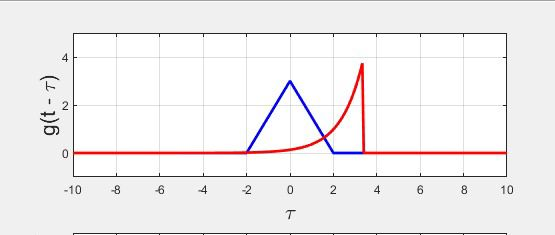
\includegraphics[scale=0.5]{figura 6}
\end{figure}
$t>2$
\begin{align}
y(t) = \overset{0}{\underset{-2}{\int }} \left[ \frac{3}{2} \tau + 3 \right] \left[ 4e^{-(t-\tau)} \right]d\tau + \overset{t}{\underset{-2}{\int }} \left[ - \frac{3}{2} \tau + 3 \right] \left[ 4e^{-(t-\tau)} \right]d\tau\\
=4 e^{-t} \left\lbrace 3 e^0 - \frac{3}{1} e^0 - \left[ \left( \frac{3}{2} (-2) +3 \right) e^{-2} - \frac{3}{2} e ^{-2} \right] + \left( - \frac{3}{2} t + 3 \right) e^t + \frac{3}{2}e^t - \left[ 3e^0 + \frac{3}{2} e^0 \right] \right\rbrace 
\end{align}
\newpage
Finalmente observamos en la gráfica el resultado de la convolucion expresado en la gráfica donde
podemos observar la contribución de cada caso.
\begin{figure} [H]
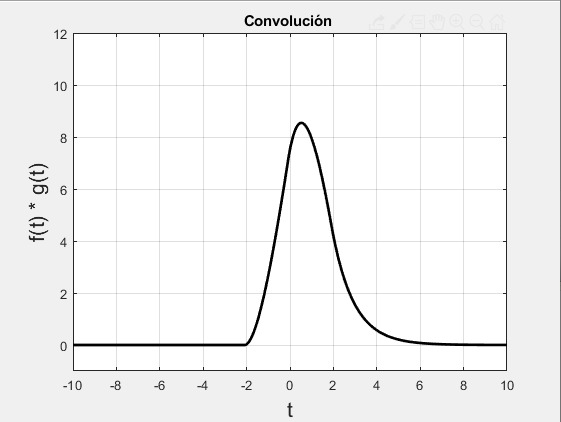
\includegraphics[scale=0.6]{figura 7}
\end{figure}


\end{document}


